\chapter{Supply and Demand}

\section{Markets and Competition}

	\begin{itemize}

	\item A \underline{market} is a group of buyers and sellers of a particular good or service.
	
	\item A \underline{competitive market} is a market with so many buyers and sellers that each has a negligible impact on the market price.
	
	\item A market is \underline{perfectly competitive} if:
	
		\begin{enumerate}
	
		\item The goods/services offered for sale are all exactly the same.
		
		\item The buyers and sellers are so numerous that no single buyer/seller has any influence on the market price.
	
		\end{enumerate}
	
	\item Buyers and sellers in perfectly competitive markets are called \underline{price takers} because they must accept the market price. 

	\end{itemize}

\section{Demand}

\subsection{The Demand Curve}

	\begin{itemize}

	\item The \underline{quantity demanded} of a good is the amount that buyers are willing and able to purchase.
	
		\begin{itemize}
		
		\item There are many determinants of quantity demanded, but the most important is the good's price.
		
		\end{itemize}
		
	\item \underline{Law of Demand}: Holding everything else constant, when the price of a good rises, the quantity demanded falls. When the price falls, the quantity demanded rises.
	
	\item A \underline{demand schedule} is a table that shows the relationship between the price of a good and the quantity demanded (holding every other determinant of quantity demanded constant).
	
	\item The \underline{demand curve} is the curve relating price and quantity demanded (holding everything else constant).
	
		\begin{itemize}
		
		\item By convention, price is plotted on the $y$-axis and quantity demanded is plotted on the $x$-axis.
		
		\end{itemize}

	\end{itemize}
	
	\begin{figure}[h]
	\underline{Ex.} Catherine's Demand Schedule and Curve
	\centering
	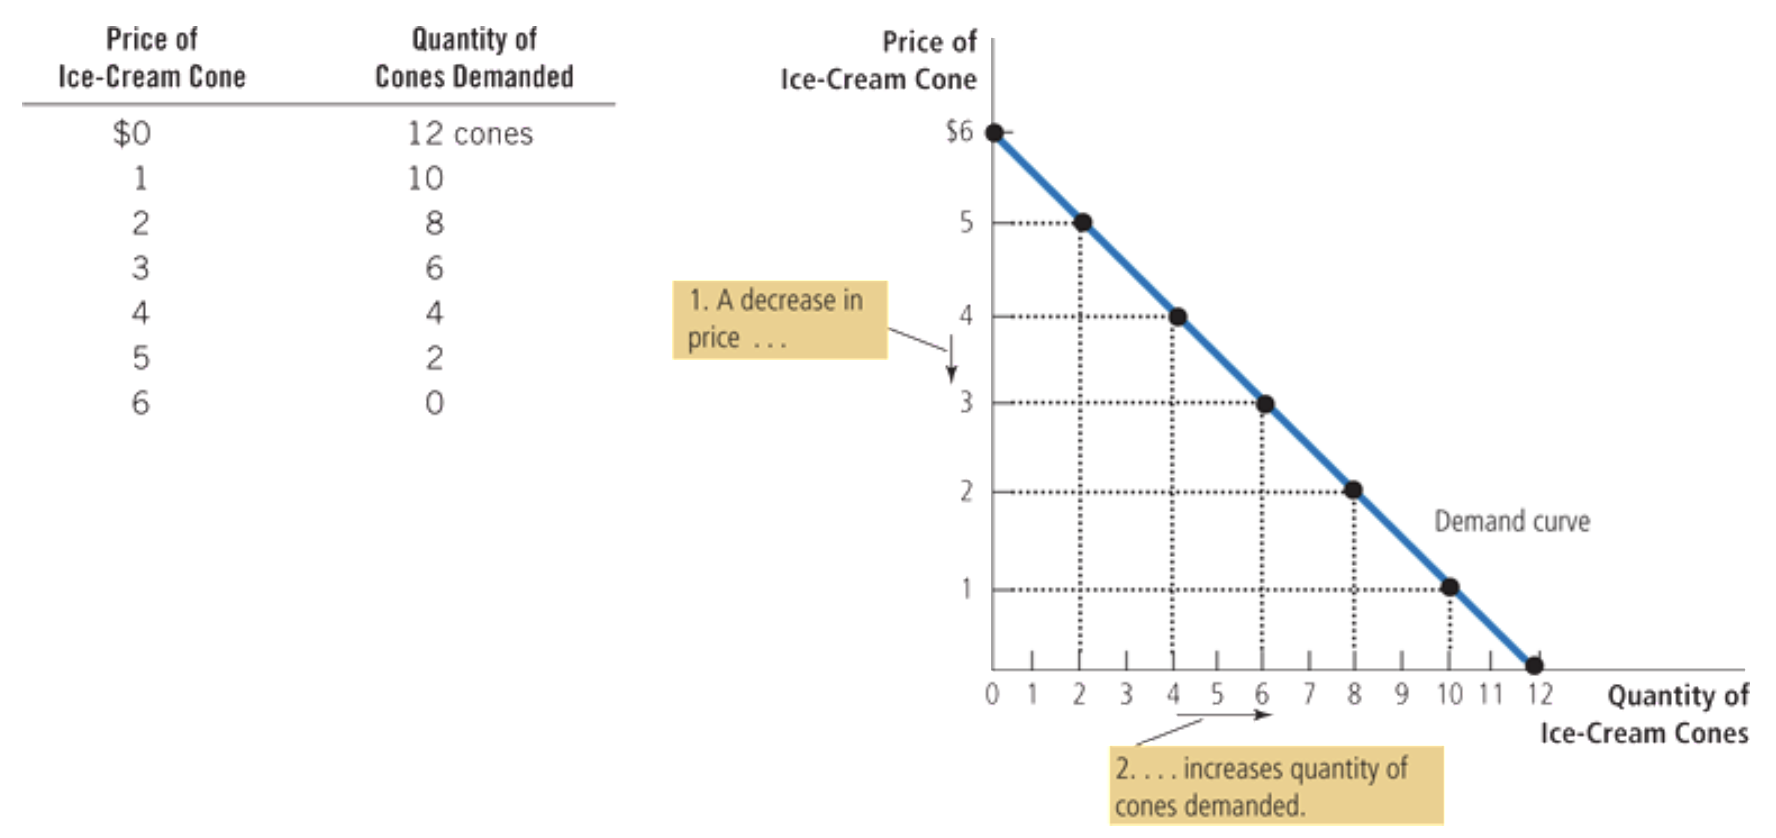
\includegraphics[width = \textwidth]{1.3.1_indiv_d_curve_sched}
	\end{figure}
	
\subsection{Market Demand}

	\begin{itemize}
	
	\item The quantity demanded in a market is the sum of every individuals' quantity demanded at each price
	
	\end{itemize}
	
	\begin{figure}[h]
	\underline{Ex.} Market Demand Schedule and Demand Curve
	\centering
	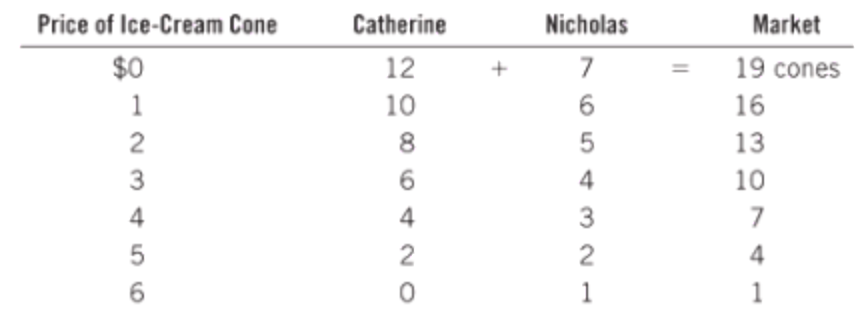
\includegraphics[width = \textwidth]{1.3.2_mkt_d_schedule}
	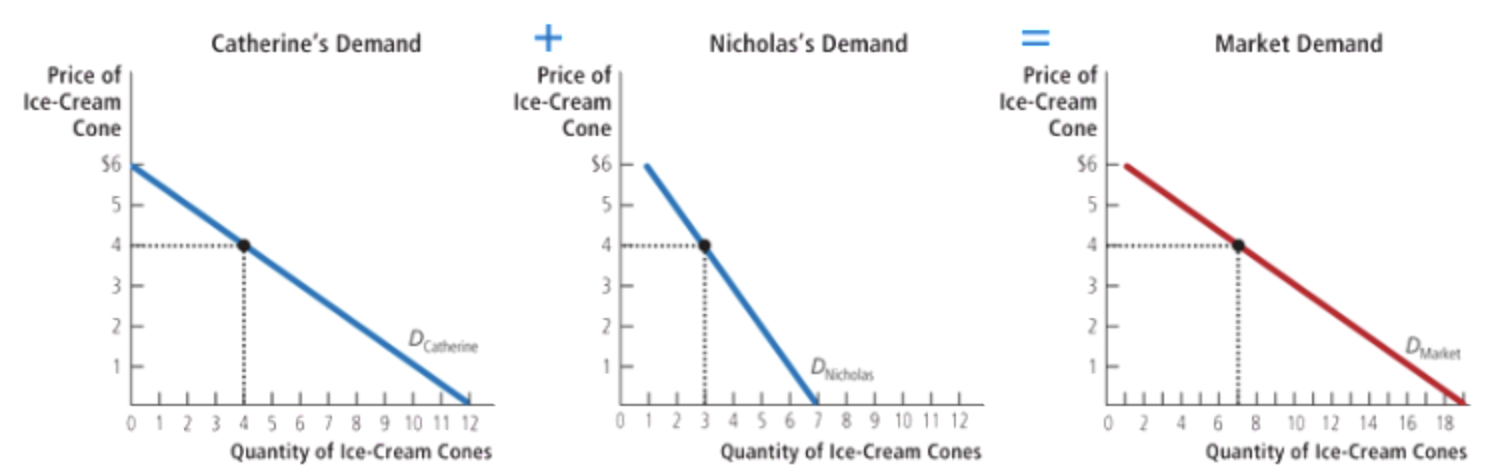
\includegraphics[width = \textwidth]{1.3.2_mkt_d_curve}
	\end{figure}
	
\subsection{Shifts in the Demand Curve}

	\begin{itemize}

	\item If a determinant of quantity demanded other than price changes, the demand curve shifts.

	\end{itemize}
	
	\underline{Variables That Shift the Demand Curve}:
	
	\begin{enumerate}
	
	\item Income: 
	
		\begin{itemize}
		
		\item Typically, when people's income falls, their demand for a good falls. If demand for a good falls when income falls, the good is called a \underline{normal good}.
		
		\item If the demand for a good rises when income falls, the good is called an \underline{inferior good}.  
		
		\end{itemize}
		
	\item Price of Related Goods:
	
		\begin{itemize}
		
		\item When a fall in the price of one good reduces the demand for another good, the two goods are called \underline{substitutes}. 
		
			\begin{itemize}
			
			\item Substitutes are often goods that are used in place of each other, e.g. ice cream and frozen yogurt
			
			\end{itemize}
		
		\item When a fall in the price of one good increases the demand for another good, the two goods are called \underline{complements}
		
			\begin{itemize}
			
			\item Complements are often goods that are used together, e.g. ice cream and ice cream cones.
			
			\end{itemize}
		
		\end{itemize}
		
	\item Tastes:
	
		\begin{itemize}
		
		\item If people's tastes (a.k.a. preferences) change, their quantity demanded will change, and the demand curve will shift.
		
		\end{itemize}
		
	\item Expectations:
	
		\begin{itemize}
		
		\item If people expect a higher price in the future, they will demand more at today's price.
		
		\item If people expect a higher income in the future, they will demand more today. 
		
		\end{itemize}
		
	\item Number of Buyers:
	
		\begin{itemize}
		
		\item An increase in the number of buyers increases demand. 
		
		\item A decrease in the number of buyers decreases demand.
		
		\end{itemize}
	
	\end{enumerate}
	
	\begin{figure}[h]
	\underline{Ex.} Shifts in the Demand Curve
	\centering
	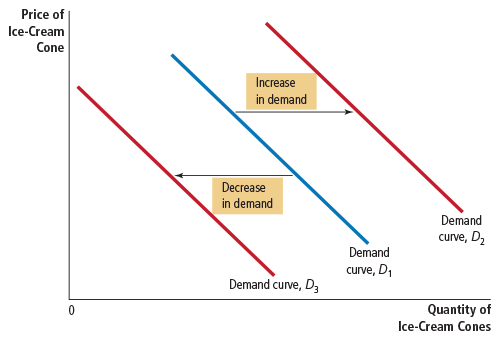
\includegraphics[width = \textwidth]{1.3.3_d_curve_shift}
	\end{figure}
	
	\underline{Warning}:
	
	\begin{itemize}
	
	\item A change in the price of a good does \textit{not} shift the demand curve for the good.
	
	\item A change in the price of a good represents a movement along the demand curve.
	
	\begin{figure}[h]
	\underline{Ex.} A Shift vs. A Movement Along
	\centering
	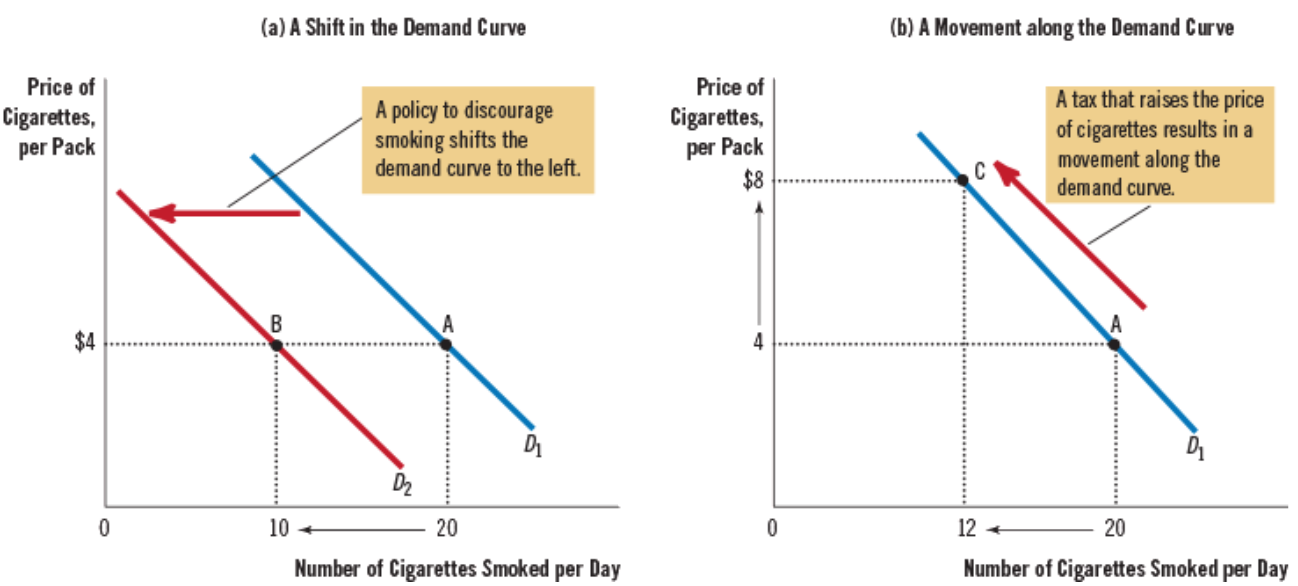
\includegraphics[width = \textwidth]{1.3.3_shift_v_mvmt_d_curve}
	\end{figure}
	
	\end{itemize}
	
\section{Supply}

\subsection{The Supply Curve}

	\begin{itemize}
	
	\item The \underline{quantity supplied} of a good is the amount that sellers are willing and able to sell.
	
		\begin{itemize}
		
		\item The most important determinant of the quantity supplied of a good is the price of the good.
		
		\end{itemize}
		
	\item \underline{Law of Supply}: Holding everything else constant, when the price of a good rises, the quantity supplied rises. When the price falls, the quantity supplied falls.
	
	\item A \underline{supply schedule} is a table that shows the relationship between the price of a good and the quantity supplied (holding every other determinant of quantity supplied constant).
	
	\item A \underline{supply curve} is the curve relating price and quantity supplied (holding everything else constant).
	
	\end{itemize}
	
	\begin{figure}[p]
	\underline{Ex.} Ben's Supply Curve
	\centering
	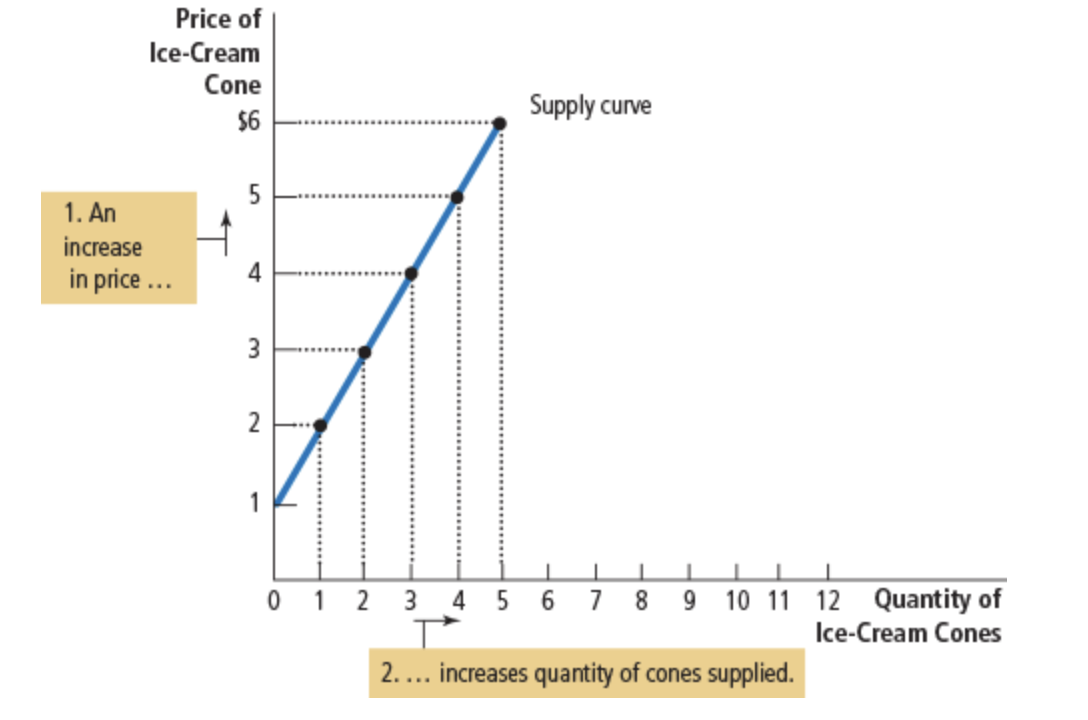
\includegraphics[width = \textwidth]{1.4.1_indiv_s_curve}
	\end{figure}
	
\subsection{Market Supply}

	\begin{itemize}
	
	\item The quantity supplied in a market is the sum of every individual's quantity supplied at each price.
	
	\begin{figure}[p]
	\underline{Ex.} Market Supply Schedule and Supply Curve
	\centering
	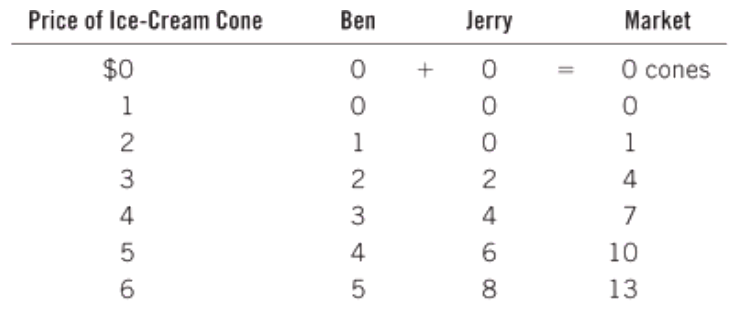
\includegraphics[width = \textwidth]{1.4.2_mkt_s_schedule}
	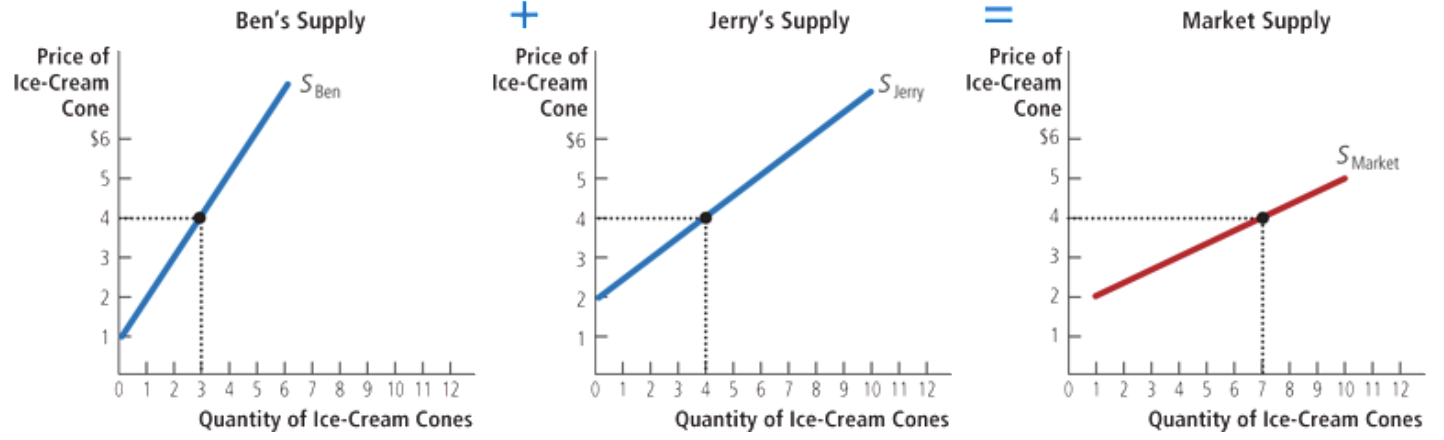
\includegraphics[width = \textwidth]{1.4.2_mkt_s_curve}
	\end{figure}
	
	\end{itemize}
	
\newpage
	
\subsection{Shifts in the Supply Curve}

	\begin{itemize}
	
	\item If a determinant of quantity supplied other than price changes, the supply curve shifts.
	
	\end{itemize}
	
	\begin{figure}[h]
	\underline{Ex.} Shifts in the Supply Curve
	\centering
	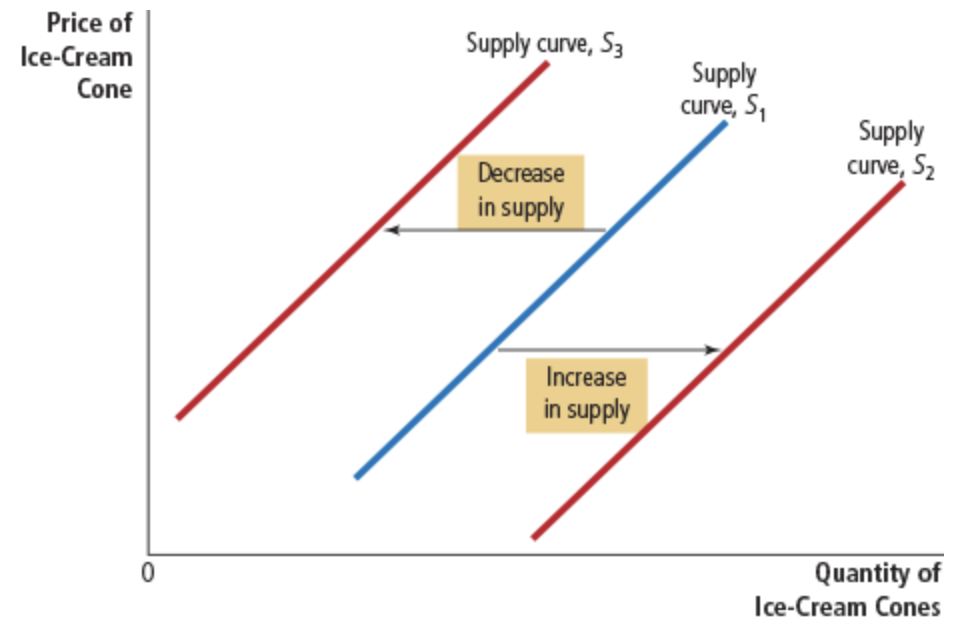
\includegraphics[width = \textwidth]{1.4.3_s_curve_shift}
	\end{figure}
	
	\underline{Variables That Shift the Supply Curve}
	
	\begin{enumerate}
	
	\item Input Prices: 
	
		\begin{itemize}
		
		\item An \underline{input} is any good or service that's used to produce another good or service.
		
		\item An increase in input prices makes production less profitable, so fewer producers are willing to supply at a given price and supply decreases.
		
		\item Similarly, a decrease in input prices will increase supply.
		
		\end{itemize}
		
	\item Technology:
	
		\begin{itemize}
		
		\item Advancement in production technology reduces costs which increases profits, so firms supply more and supply increases.
		
		\item Similarly, a decline in production technology will decrease supply.
		
		\end{itemize}
		
	\item Expectations:
		
		\begin{itemize}
		
		\item If firms expect higher prices in the future, they will postpone some production, and supply in the present will decrease.
		
		\item If firms expect lower prices in the future, they will fast forward its production, so supply in the present will increase.
		
		\end{itemize}
		
	\item Number of Sellers
	
		\begin{itemize}
	
		\item An increase in the number of sellers increases supply.
		
		\item A decrease in the number of sellers decreases supply.
		
		\end{itemize}
	
	\end{enumerate}
	
	\underline{Warning}:
	
	\begin{itemize}
	
	\item A change in the price of a good does \textit{not} shift the supply curve for the good.
	
	\item A change in the price of a good represents a movement along the supply curve.
	
	\end{itemize}
	
\section{Supply and Demand Together}

\subsection{Equilibrium}

	\begin{itemize}

	\item A market is in \underline{equilibrium} if quantity supplied equals quantity demanded.
		
	\item Equilibrium occurs at the point where the supply and demand curves intersect.
	
	\item The quantity at equilibrium is called the \underline{equilibrium quantity}.
	
	\item The price at equilibrium is called the \underline{equilibrium price} or the \underline{market-clearing price}.
	
	\begin{figure}[h]
	\underline{Ex.} Market Equilibrium
	\centering
	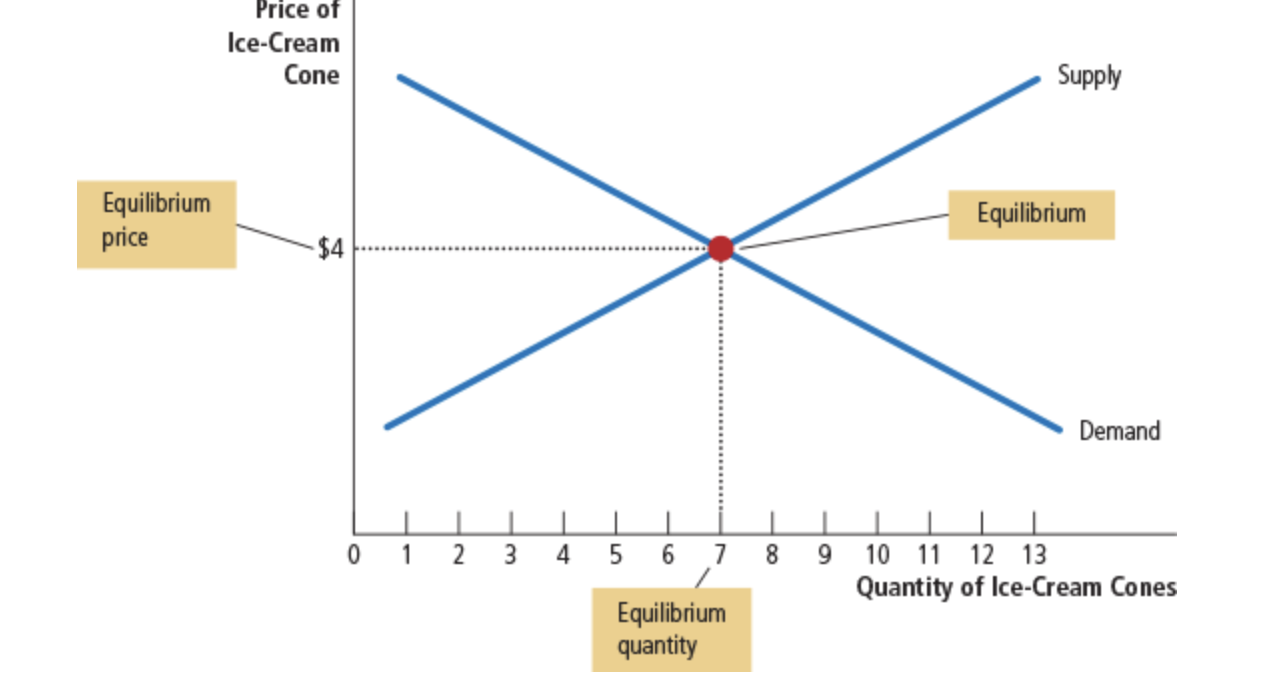
\includegraphics[width = \textwidth]{1.5.1_mkt_eq}
	\end{figure}
	
	\item There is a \underline{surplus} of a good when the quantity supplied exceeds the quantity demanded.
	
		\begin{itemize}
		
		\item Sellers can't sell all of their goods, so they cut the price. That moves the market back towards equilibrium.
		
		\end{itemize}
		
	\item There is a \underline{shortage} when the quantity demanded exceeds the quantity supplied.
	
		\begin{itemize}
		
		\item Buyers can't buy as much as they want, so they bid up the price. That moves the market back towards equilibrium. 
		
		\end{itemize}
		
	\item In both cases, markets tend towards equilibrium.
		
	\begin{figure}[h]
	\underline{Ex.} A Shortage and A Surplus
	\centering
	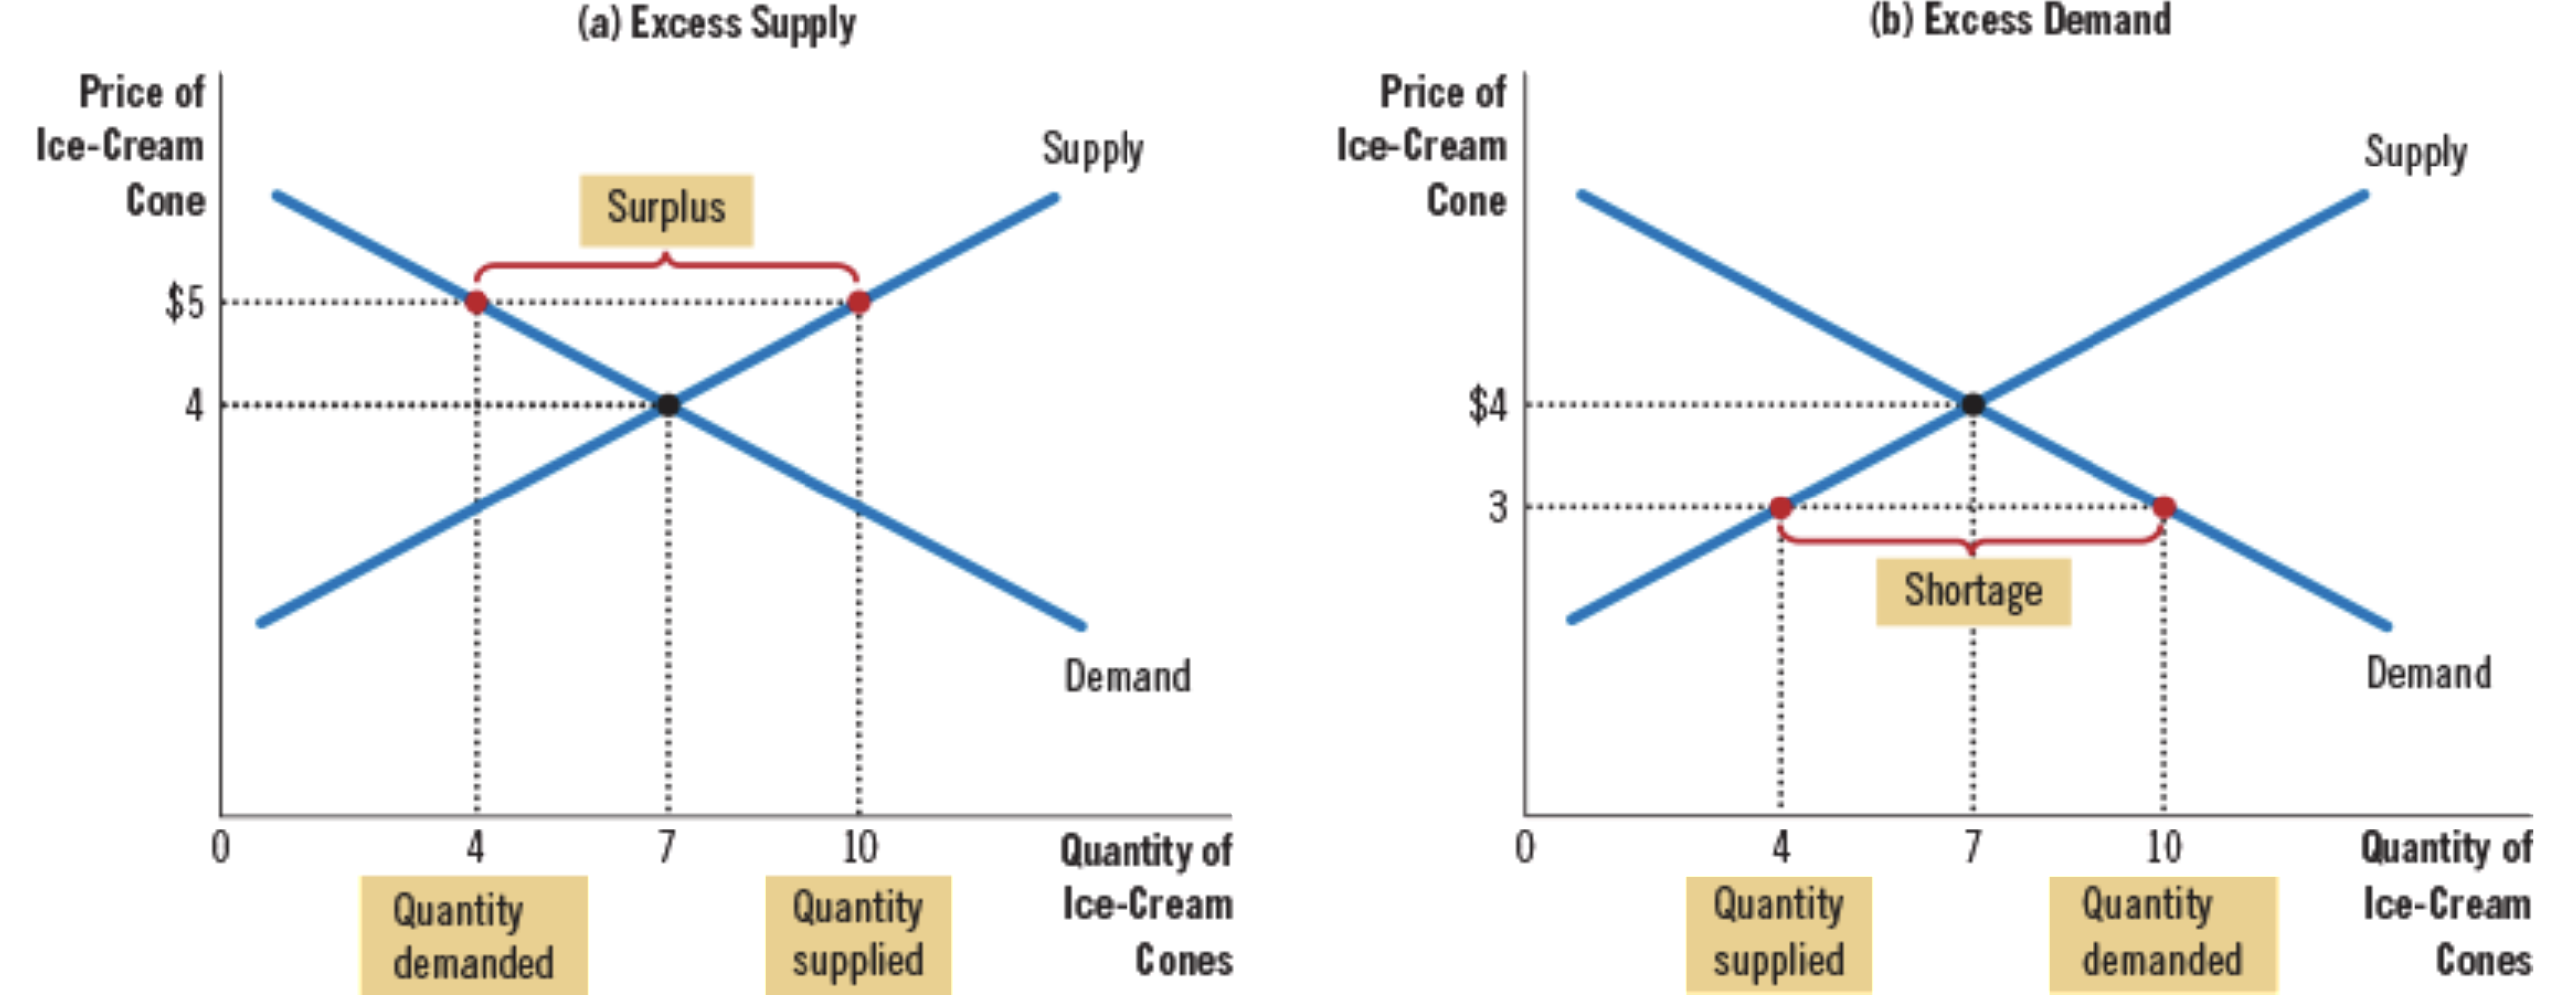
\includegraphics[width = \textwidth]{1.5.1_mkt_diseq}
	\end{figure}
	
	\end{itemize}
	
\subsection{Analyzing Changes in Equilibrium}

	To analyze an event's effect on equilibrium, follow three steps:
	
	\begin{enumerate}
	
	\item Determine whether the event shifts supply, demand, or both.
	
	\item Determine the direction of the shift.
	
	\item Draw a supply-and-demand diagram to see how the new equilibrium compares to the old. 
	
	\end{enumerate}
	
	\noindent \underline{Ex.} How does a heat wave affect equilibrium in the market for ice cream?
	
	\begin{enumerate}
	
	\item Hot weather increases people's preference for ice cream, so the demand curve shifts. Supply remains unchanged.
	
	\item An increased preference for ice cream will shift the curve to the right. 
	
	\item Equilibrium price and quantity both increase. 
	
	\begin{figure}[h]
	The Market for Ice Cream During a Heat Wave
	\centering
	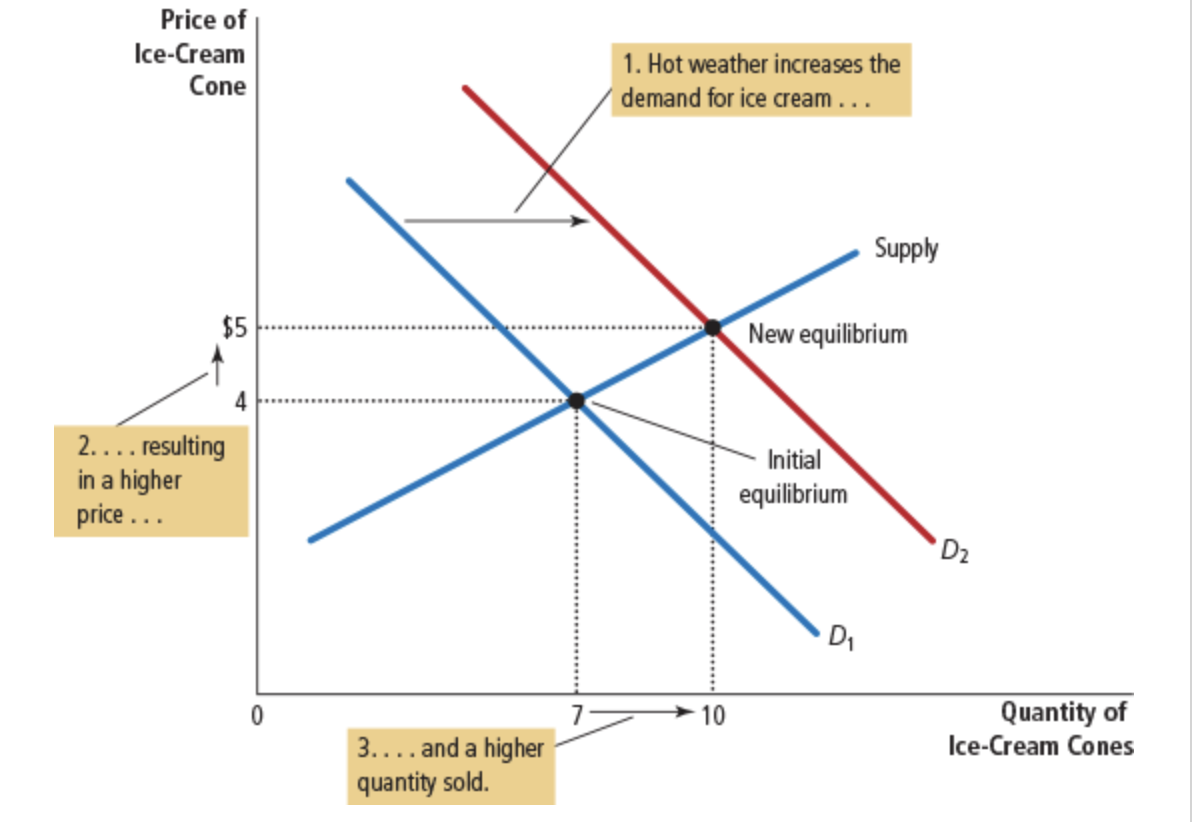
\includegraphics[width = 0.78\textwidth]{1.5.2_d_shift}
	\end{figure}
	
	\end{enumerate}
	
	\newpage
	
	\noindent \underline{Ex.} A hurricane destroys part of the sugarcane crop and drives up the price of sugar. What happens to equilibrium in the market for ice cream?
	
	\begin{enumerate}
	
	\item The price of an input changed, so the supply curve shifts. Demand remains unchanged.
	
	\item Higher input prices will shift the curve to the left. 
	
	\item Equilibrium price increases and equilibrium quantity decreases. 
	
	\begin{figure}[h]
	The Market for Ice Cream After a Hurricane
	\centering
	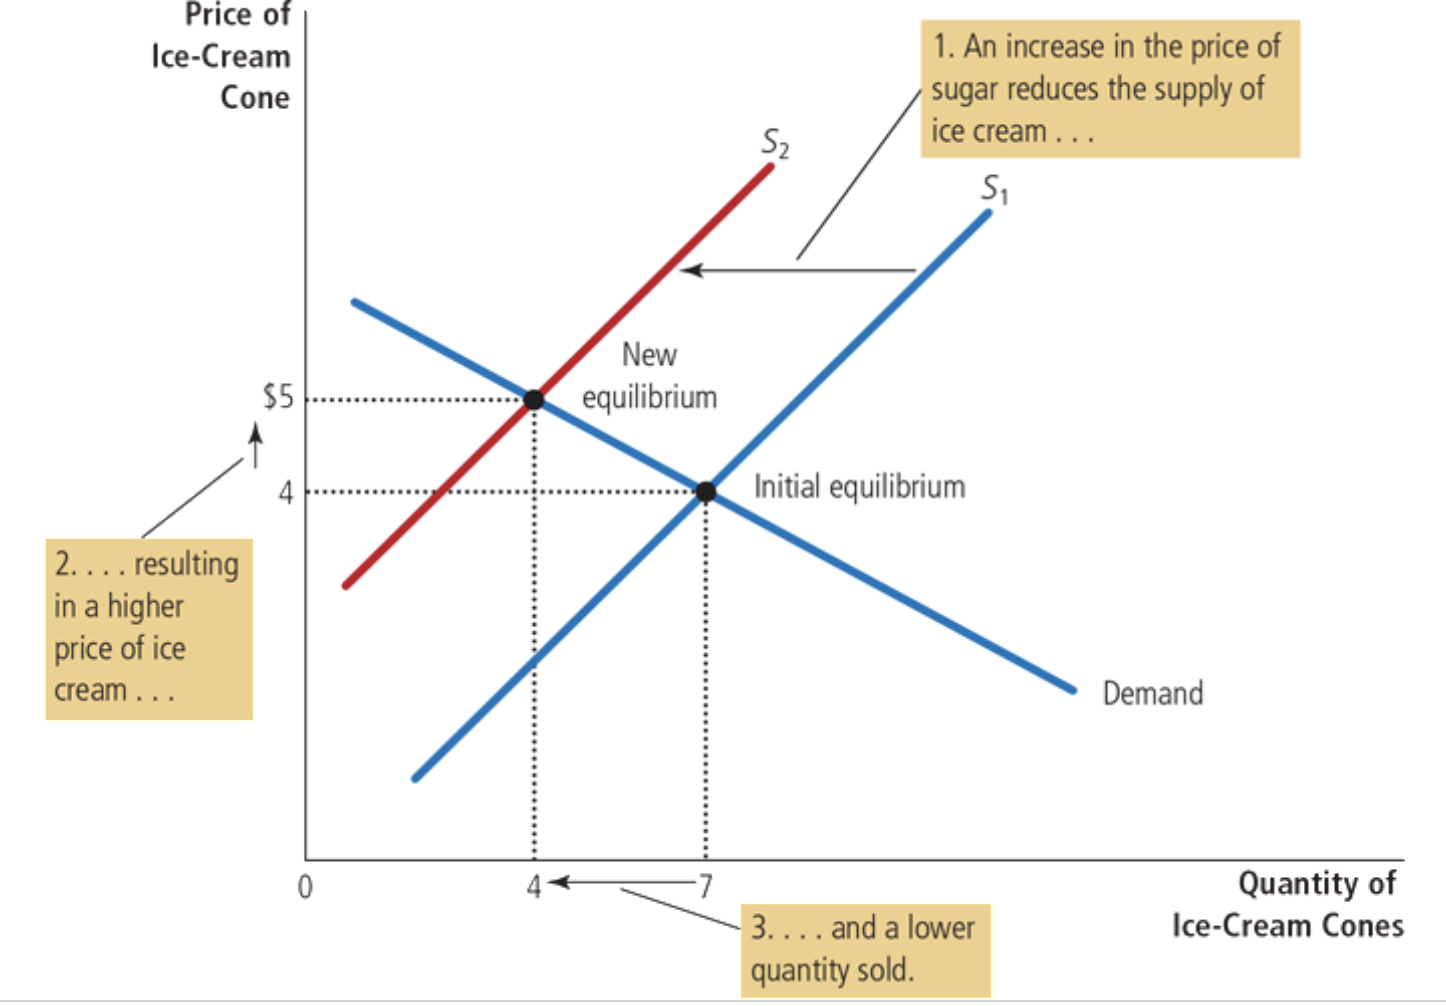
\includegraphics[width = 0.78\textwidth]{1.5.2_s_shift}
	\end{figure}
	
	\end{enumerate}
	
	\newpage
	
	\noindent \underline{Ex.} The heat wave and hurricane happen in the same summer. What happens to equilibrium?
	
	\begin{enumerate}
	
	\item Demand and supply both shift for the same reasons as above.
	
	\item Demand shifts right, and supply shifts left for the same reasons as above.
	
	\item The equilibrium price increases. The change in equilibrium quantity is ambiguous. It depends on the relative sizes of the shifts. 
	
	\begin{figure}[h]
	The Market for Ice Cream During a Heat Wave and After a Hurricane
	\centering
	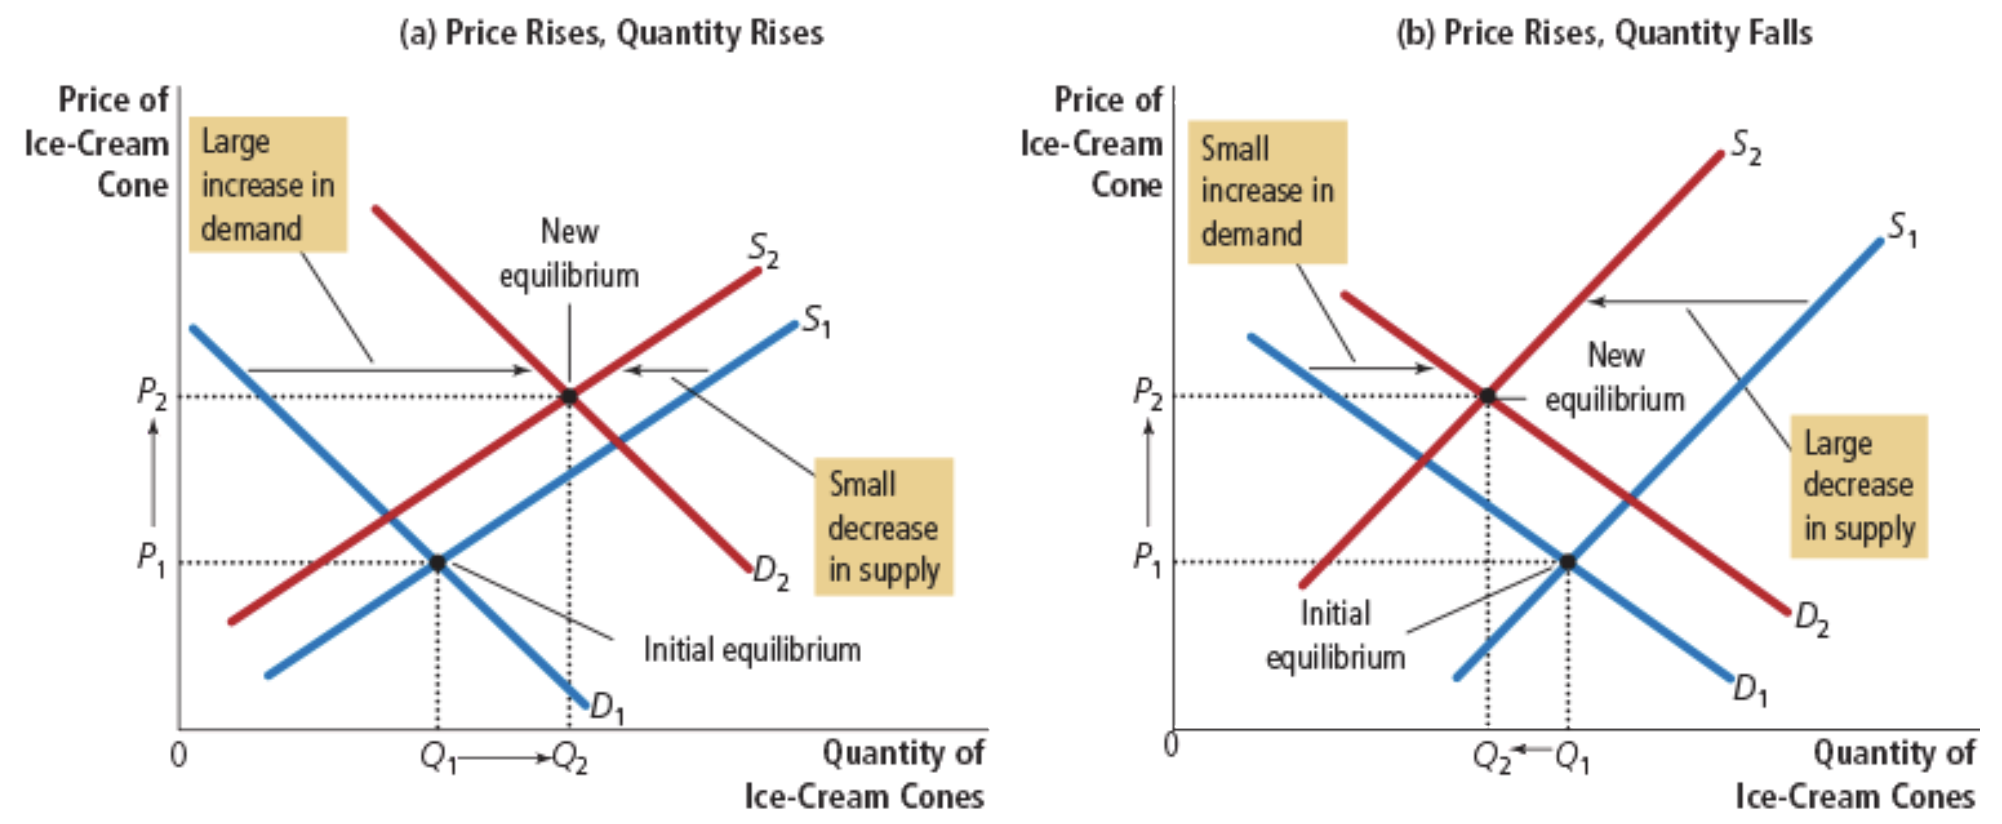
\includegraphics[width = \textwidth]{1.5.2_both_shift}
	\end{figure}
	
	\end{enumerate}



